% =====================================================================
%  AMLBT Project Report -- HridayTwin
%  IEEE conference format (IEEEtran). Compiles on Overleaf as-is:
%  upload main.tex + the figures/ folder into your copy of the course
%  template, or run `latexmk -pdf main.tex` locally.
% =====================================================================
\documentclass[conference]{IEEEtran}
\IEEEoverridecommandlockouts
\usepackage{cite}
\usepackage{amsmath,amssymb,amsfonts}
\usepackage{graphicx}
\usepackage{booktabs}
\usepackage{float}
\usepackage{multirow}
\usepackage{textcomp}
\usepackage{xcolor}
\usepackage{tikz}
\usetikzlibrary{positioning,arrows.meta,fit,calc}
\usepackage[hidelinks]{hyperref}
\usepackage{url}
\def\BibTeX{{\rm B\kern-.05em{\sc i\kern-.025em b}\kern-.08em
    T\kern-.1667em\lower.7ex\hbox{\sc e}\kern-.125em X}}

% ---------------- edit these before submitting ----------------------
\newcommand{\RepoURL}{https://github.com/Mazekerr/hridaytwin-amlbt}
\newcommand{\StudentIDs}{\{B2026013, B2026022\}}  % <-- replace with your GIM IDs
% --------------------------------------------------------------------

\begin{document}

\title{HridayTwin: A Personal Digital Twin and Fused Risk Engine for Predicting Adverse Cardiometabolic Events in Indian Adults with Diabetes and Hypertension}

\author{\IEEEauthorblockN{Dhruvik Sorathiya, Kruparth Pandya}
\IEEEauthorblockA{Goa Institute of Management\\
Big Data Analytics\\
Student IDs: \StudentIDs\\
Email: \{dhruvik.sorathiya2026b, kruparth.pandya2026b\}@gim.ac.in}}

\maketitle

\begin{abstract}
Adults with type~2 diabetes and hypertension in India are seen in short outpatient visits weeks or months apart, while the warning signs of an emergency build up at home in between. Remote-monitoring programmes now collect home glucose, blood pressure (BP), step and pill-box data, but care teams lack a way to decide whom to call, why, and what to change. We build HridayTwin, a two-part machine learning system. A per-patient Bayesian state-space model (the \emph{digital twin}) starts from the clinic record and is updated daily by a Kalman filter, learning how strongly each patient's medicines, salt and activity move their glucose and BP. A gradient-boosted risk engine fuses 59 record and home-device features to predict any of four adverse events in the next 14 days, and scores 90-day what-if simulations of candidate care plans rolled out on the twin. On a mechanistic synthetic cohort of 1{,}200 patients followed for 180 days, the fused model reaches an AUROC of 0.726 against 0.708 for the clinic record alone ($p=0.008$, patient-level bootstrap) and 0.615 for threshold rules, with the largest gain for severe hypoglycaemia (0.943 vs.\ 0.907). At a budget of 10 alerts per 100 patient-weeks it gives a median of 7 days' warning. We report the negative findings alongside and release all code and data for reproduction.
\end{abstract}

\begin{IEEEkeywords}
Digital twin, Kalman filter, gradient boosting, remote patient monitoring, clinical risk prediction, diabetes, hypertension, India
\end{IEEEkeywords}

% =====================================================================
\section{Introduction}
India has an estimated 101 million adults with diabetes and 315 million with hypertension, and the two conditions frequently occur together \cite{anjana2023}. Their care is organised around brief outpatient (OPD) visits. Between visits, the clinician sees nothing, yet most avoidable emergencies (severe hypoglycaemia, hyperglycaemic crises, hypertensive emergencies and acute cardiovascular events) are preceded by days of visible signals: missed doses, rising home BP, low glucose readings on a fasting day, or a resting-heart-rate spike from an infection.

The business problem is therefore one of \emph{prioritisation under a fixed care-team capacity}. Hospital chains, digital-health companies, insurers and employer wellness programmes increasingly run remote-monitoring programmes that collect these signals, but a care coordinator faced with thousands of readings per day cannot tell who needs a call this week. A tool that ranks patients by short-term risk, explains the ranking and suggests a tested change of plan turns a passive data stream into a call list. The value is measured in avoidable admissions, coordinator minutes per patient, and the quality metrics (HbA1c and BP control) that payers and accreditation bodies track. The same output serves four users: the coordinator gets a ranked worklist, the physician gets personal drug-response estimates and guarded plan options, the patient gets fewer emergencies, and the programme manager gets fewer avoidable admissions.

\subsection{Scope and Objectives}
The project aims to build and rigorously evaluate a decision-support system that answers three questions for a care team each week: \emph{who} is likely to have an adverse event in the next 14 days and why; \emph{how} this patient actually responds to their medicines, salt and activity; and \emph{what} change of plan would lower their risk. The objectives are to:
\begin{itemize}
\item establish the business relevance of between-visit risk triage for Indian chronic-care programmes;
\item design an original architecture that separates a generative patient twin from a discriminative risk engine;
\item quantify, with leakage-safe validation, how much home-device data adds over the clinic record; and
\item release data, code and tests so every number is reproducible with one command.
\end{itemize}

\section{Project Submission Details}
The team consists of Dhruvik Sorathiya and Kruparth Pandya (Big Data Analytics, Goa Institute of Management). The final code, the cleaned modelling dataset and this report's source are in the public repository \url{\RepoURL}. Steps to replicate the core results are in Section~\ref{sec:repro}, and the AI use declaration is in Section~\ref{sec:ai}.

% =====================================================================
\section{Related Work}
\subsection{Digital twins in medicine} A digital twin is a computational model of an individual that is kept in sync with that individual's data and used to simulate interventions \cite{bjornsson2020}. In cardiology, twins have been argued to combine mechanistic and statistical models for precision care \cite{corral2020}; a recent scoping review finds that most health twins remain conceptual or organ-level, with few that update continuously from routine data or are evaluated against outcomes \cite{katsoulakis2024}. HridayTwin is a deliberately simple, identifiable twin that runs on the daily summaries low-cost Indian home devices produce. In diabetes, simulators such as the UVA/Padova model of glucose--insulin dynamics are widely used for in-silico testing of type~1 control algorithms \cite{man2014}; HridayTwin instead targets type~2 diabetes with hypertension and learns each patient's response from home data.

\subsection{Risk prediction from health records} Deep and tree-based models trained on electronic health records (EHRs) predict admissions and deterioration well \cite{rajkomar2018}, and gradient boosting outperformed logistic regression for inpatient hypoglycaemia \cite{ruan2020}. These models use the record alone and score hospital stays; they do not use the home data that exists between outpatient visits, and they do not say what to change.

\subsection{State-space models and boosting} The Kalman filter \cite{kalman1960} gives exact Bayesian updates for linear-Gaussian models, with uncertainty that grows when data are missing \cite{durbin2012}. Gradient boosting \cite{friedman2001}, in its histogram-based form \cite{ke2017,pedregosa2011}, is a strong default for tabular data with missing values, and SHAP values provide per-prediction explanations \cite{lundberg2017}.

\subsection{Our contribution} We differ from prior work in four ways: (i) the twin's prior comes from the clinic record and published drug effects, and its posterior from home data, so it personalises without per-patient training; (ii) the twin is \emph{generative} and the risk engine \emph{discriminative}, so simulated futures are scored by exactly the model that scores real patients; (iii) the Indian calendar (Ekadashi, Navratri and Shravan fasts, Diwali, the monsoon) enters the model and the simulator; and (iv) we test the value of home data with ablations, a patient-level bootstrap, a temporal hold-out, a label-permutation control and a seed sweep, and report what did not work.

% =====================================================================
\section{Methodology}

\subsection{Data}
Paired EHR and daily home-device data for Indian patients are not publicly available, so we wrote a mechanistic generator (in the spirit of Synthea \cite{walonoski2018}) whose parameters come from published Indian and trial evidence: prevalence \cite{anjana2023}, the HbA1c--mean glucose relation \cite{nathan2008}, drug effect sizes, infection as a cardiovascular trigger \cite{kwong2018} and fasting guidance (Ramadan guidelines, the closest evidence-based analogue for Hindu fasts) \cite{hassanein2022}. Each simulated patient has a \emph{hidden} physiology (drug response, salt and activity sensitivity) that evolves daily under medicines, adherence, diet, illness, monsoon and fasting. Events are drawn from the hidden state; the models see only noisy, gappy device readings, so labels cannot be read off any input column. Table~\ref{tab:data} summarises the cohort.

\begin{table}[H]
\caption{Synthetic cohort (seed 2026)}
\label{tab:data}
\centering
\footnotesize
\begin{tabular}{@{}ll@{}}
\toprule
Patients $\times$ days & 1{,}200 $\times$ 180 (216{,}000 patient-days)\\
Demographics & age 30--84, 54\% male, five regions\\
Conditions & 76\% type 2 diabetes, 71\% hypertension\\
EHR fields & 26 (labs, diagnoses, medicine classes, fasting, CGM)\\
Daily stream & steps, resting HR, HRV, sleep, glucose, BP,\\
 & pill-box doses, salt and carbohydrate log, weight\\
Missingness & wearable 22\%, glucose 48\%, home BP 55\%,\\
 & pill-box 15\%, diet log 62\% of days\\
Adverse events & 724 (310 CV, 168 hyperglycaemic,\\
 & 148 hypertensive, 98 severe hypoglycaemia)\\
Modelling rows & 23{,}710 weekly check-ins, 4.5\% positive\\
\bottomrule
\end{tabular}
\end{table}

\textit{Preprocessing.} The long patient-day table is pivoted to (patient $\times$ day) arrays. Missing readings stay missing (no imputation): the twin skips them and the gradient-boosted trees route them natively, while explicit counts of readings per window let the model learn that silence is itself a signal. A prediction is made every 7 days after a 28-day warm-up, on days the patient is not in hospital. Each row has 27 EHR features, 29 causal stream features (3/7/14/28-day means, minima, maxima, trends and counts, e.g.\ missed doses or readings below 70\,mg/dL) and 3 calendar features (fast and feast days in the next 14 days, monsoon). Every window ends on the prediction day; a unit test scrambles all later data and checks that no feature changes. The label is any adverse event in the following 14 days. The cleaned modelling table is released in the repository.

\subsection{Models and Techniques}
\begin{figure}[H]
\centering
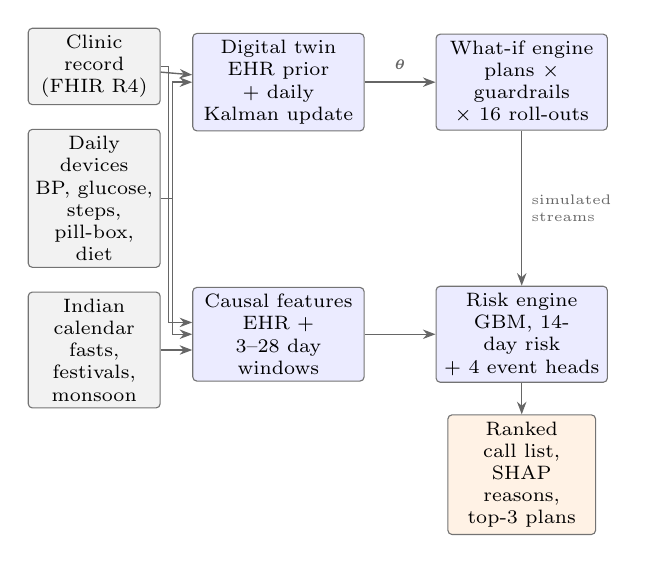
\begin{tikzpicture}[font=\scriptsize, node distance=3mm and 4mm,
  box/.style={draw=black!55, rounded corners=1.5pt, align=center, inner sep=2.5pt, minimum height=6.5mm},
  inb/.style={box, fill=black!5, text width=15mm},
  core/.style={box, fill=blue!8, text width=20mm},
  outb/.style={box, fill=orange!10, text width=17mm},
  arr/.style={-{Stealth[length=1.6mm]}, black!60, line width=0.5pt}]
\node[inb] (ehr) {Clinic record\\(FHIR R4)};
\node[inb, below=of ehr] (dev) {Daily devices\\BP, glucose, steps,\\pill-box, diet};
\node[inb, below=of dev] (cal) {Indian calendar\\fasts, festivals,\\monsoon};
\node[core, right=of ehr, yshift=-2mm] (twin) {Digital twin\\EHR prior + daily\\Kalman update};
\node[core, right=of cal, yshift=2mm] (feat) {Causal features\\EHR + 3--28 day\\windows};
\node[core, right=9mm of feat] (gbm) {Risk engine\\GBM, 14-day risk\\+ 4 event heads};
\node[core, right=9mm of twin] (sim) {What-if engine\\plans $\times$ guardrails\\$\times$ 16 roll-outs};
\node[outb, below=4mm of gbm] (ui) {Ranked call list,\\SHAP reasons,\\top-3 plans};
\draw[arr] (ehr) -- (twin);
\draw[arr] (dev.east) -- ++(1.5mm,0) |- (twin.west);
\draw[arr] (dev.east) -- ++(1.5mm,0) |- (feat.west);
\draw[arr] (ehr.east) -- ++(1mm,0) |- ([yshift=1.5mm]feat.west);
\draw[arr] (cal) -- (feat.west |- cal);
\draw[arr] (twin) -- node[above=1pt, font=\tiny]{$\boldsymbol\theta$} (sim);
\draw[arr] (feat) -- (gbm);
\draw[arr] (sim.south) -- node[right, font=\tiny, align=left]{simulated\\streams} (gbm.north);
\draw[arr] (gbm) -- (ui);
\end{tikzpicture}
\caption{HridayTwin architecture: The twin \emph{simulates}; the risk engine \emph{judges} both real and simulated futures with the same model. FHIR R4 is the HL7 Fast Healthcare Interoperability Resources standard.}
\label{fig:arch}
\end{figure}

Fig.~\ref{fig:arch} shows the system. It has three components.

\textbf{1) Digital twin:} For each patient, two linear-Gaussian state-space models describe daily mean glucose and home systolic BP:
\begin{equation}
y_t = \mathbf{x}_t^{\top}\boldsymbol{\theta}_t + \varepsilon_t,\quad \boldsymbol{\theta}_t=\boldsymbol{\theta}_{t-1}+\boldsymbol{\eta}_t,
\label{eq:ssm}
\end{equation}
with $\varepsilon_t\sim\mathcal N(0,\sigma^2)$ and $\boldsymbol\eta_t\sim\mathcal N(\mathbf 0,Q)$. The inputs $\mathbf x_t$ are an intercept, pill-box adherence, steps above the patient's own 28-day baseline, carbohydrate (glucose) or salt (BP) intake, and an illness proxy (resting heart rate above baseline), each passed through a first-order physiological lag. The coefficients $\boldsymbol\theta$ are the patient's personal physiology, e.g.\ ``her medicines lower her glucose by $41\pm9$\,mg/dL when taken''; the slow random walk lets them drift. The prior comes from the EHR: the glucose intercept starts at the estimated average glucose $\mathrm{eAG}=28.7\,\mathrm{HbA1c}-46.7$ \cite{nathan2008} adjusted for the current medicines, and the drug coefficient at minus the sum $L$ of published average effects of those medicines, with a wide prior SD ($0.6L$) so data can move it. Each day the Kalman filter \cite{kalman1960} gives a one-step forecast $\hat y_t$ with variance $S_t$ before the reading arrives, then updates
\begin{equation}
K_t=\frac{P_{t|t-1}\mathbf x_t}{S_t},\;\;
\boldsymbol\theta_{t|t}=\boldsymbol\theta_{t|t-1}+K_t\,(y_t-\hat y_t),\;\;
z_t=\frac{y_t-\hat y_t}{\sqrt{S_t}},
\end{equation}
with $S_t=\mathbf x_t^\top P_{t|t-1}\mathbf x_t+\sigma^2$ and $P_{t|t-1}=P_{t-1|t-1}+Q$. Missing days skip the update, so uncertainty grows honestly. We chose this model over a neural ODE because it is identifiable from sparse home data, every coefficient has a clinical meaning, and it updates all patients in milliseconds.

\textbf{2) Risk engine:} A histogram gradient-boosting (GBM) classifier \cite{friedman2001,ke2017} (scikit-learn \cite{pedregosa2011}; 250 iterations, learning rate 0.04, 12 leaves, at least 120 samples per leaf, L2 penalty 3) predicts the composite 14-day event from the 59 fused features, and four further heads predict each event type. Boosted trees were chosen because they handle missing values natively, capture interactions such as ``sulfonylurea $\times$ fasting day'' without hand-crafting, and are calibrated well enough to set an alert threshold. Baselines are an EHR-only model, a stream-only model, a fused logistic regression ($C=0.3$) and a points score a clinic could apply to the same readings without a model (7-day maximum SBP $\ge170$ or glucose $\ge300$, any reading $<70$\,mg/dL, adherence below 50\%, prior CVD, age $\ge65$). Per-prediction explanations use SHAP TreeExplainer \cite{lundberg2017}.

\textbf{3) What-if engine:} For each patient, candidate plans cross one medicine change (add a drug class, up-titrate, switch, or a fasting-day dose plan) with $+2{,}000$ steps/day, $-3$\,g salt/day and adherence support. Clinical guardrails remove unsafe plans (e.g.\ SGLT2 inhibitor only if eGFR $\ge20$, metformin only if eGFR $\ge30$, no second RAAS blocker) and attach cautions. Each remaining plan is rolled forward 90 days on the twin 16 times with the patient's own learned coefficients, noise and data gaps and the real future calendar (Navratri, Diwali), using common random numbers so plans differ only by the plan. The simulated streams go through the same feature builder and risk engine; plans are ranked by mean simulated 14-day risk plus a small burden penalty, and the top three are shown \emph{for clinician review}.

\subsection{Evaluation Metrics}
All models use the same 5-fold \texttt{GroupKFold} split by patient, so no patient is in both training and test data. \emph{AUROC} measures ranking (who to call first). Because events are rare (4.5\%), we also report \emph{AUPRC} \cite{saito2015}. A care team acts on probabilities, so we check calibration with the Brier score and expected calibration error (ECE) \cite{vancalster2019}. Operationally, the threshold is set by an \emph{alert budget} of 10 alerts per 100 patient-weeks rather than at 0.5; at that point we report sensitivity, positive predictive value (PPV), lift over the base rate and the median lead time before the event. Differences between models are tested with a 1{,}000-resample patient-level cluster bootstrap. Further checks are a temporal and patient hold-out (train before day 97, test from day 111 on unseen patients), a label-permutation control, a within-patient AUROC (can the model tell \emph{which week} is dangerous?), a three-seed rerun of the whole pipeline, and, for the twin, the correlation of its learned drug response with each patient's hidden true response.

% =====================================================================
\section{Results}

\begin{figure*}[t]
\centering
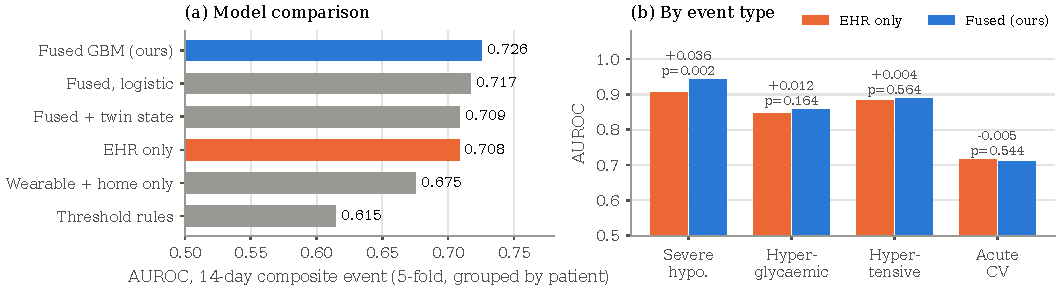
\includegraphics[width=\textwidth]{figures/fig_performance.pdf}
\caption{(a) Out-of-fold AUROC for the composite 14-day event. (b) AUROC per event type, with the fused$-$EHR difference and its bootstrap $p$-value.}
\label{fig:perf}
\end{figure*}

\begin{table}[H]
\caption{Composite 14-day event, 5-fold patient-grouped CV}
\label{tab:models}
\centering
\footnotesize
\begin{tabular}{@{}lcccc@{}}
\toprule
Model & AUROC & AUPRC & Brier & ECE\\
\midrule
\textbf{Fused EHR + stream (GBM)} & \textbf{0.726} & \textbf{0.111} & \textbf{0.0416} & \textbf{0.0053}\\
Fused, logistic regression & 0.717 & 0.106 & -- & --\\
Fused + twin-state features & 0.709 & 0.106 & 0.0418 & 0.0068\\
EHR only & 0.708 & 0.096 & 0.0423 & 0.0104\\
Wearable + home devices only & 0.675 & 0.098 & 0.0421 & 0.0072\\
Threshold rules & 0.615 & 0.072 & -- & --\\
\bottomrule
\end{tabular}
\end{table}

\subsection{Risk prediction} Table~\ref{tab:models} and Fig.~\ref{fig:perf}(a) compare the models. The fused model is best on every metric. Its AUROC gain over the clinic record alone is modest but significant ($+0.017$, 95\% CI $[+0.004,+0.032]$, $p=0.008$); over threshold rules it is $+0.111$ ($p\le0.001$). The fused logistic regression is close ($+0.009$, $p=0.23$), so most of the gain comes from the data, not the learner. The model is well calibrated (ECE 0.005; Fig.~\ref{fig:twin}(b)). The label-permutation control gives 0.515, as it should if nothing leaks. On the stricter temporal hold-out ($n=9{,}495$) the fused model scores 0.686 against 0.681, a gain of only $+0.005$, so the advantage shrinks under the stricter test. Rerunning the whole pipeline on seeds 2026, 11 and 37 gives fused AUROCs of 0.726, 0.728 and 0.726, and fused beats EHR-only on all three (Table~\ref{tab:seeds}; mean gain $+0.012\pm0.005$).

\begin{table}[H]
\caption{Seed robustness: whole pipeline rerun (new cohort, twin and models)}
\label{tab:seeds}
\centering
\footnotesize
\setlength{\tabcolsep}{4pt}
\begin{tabular}{@{}lcccc@{}}
\toprule
Seed & Base rate & EHR only & Fused & Gain\\
\midrule
2026 & 4.5\% & 0.708 & 0.726 & $+0.017$\\
11 & 4.4\% & 0.716 & 0.728 & $+0.012$\\
37 & 4.2\% & 0.717 & 0.726 & $+0.008$\\
\midrule
Mean$\pm$SD & -- & $0.714\pm0.005$ & $0.727\pm0.001$ & $+0.012\pm0.005$\\
\bottomrule
\end{tabular}
\end{table}

\subsection{Where home data helps} Fig.~\ref{fig:perf}(b) and Table~\ref{tab:events} split the result by event. Daily data add most where physiology moves fast and is measured directly: severe hypoglycaemia rises from 0.907 to 0.943 ($p=0.002$), driven by glucose lows, fasting days and missed meals. Gains for hyperglycaemic and hypertensive crises are small and not significant, and acute cardiovascular events are not improved (0.711 vs.\ 0.716); they remain driven by baseline risk in the record. The hypoglycaemia gain survives a Bonferroni correction across the four event types ($0.002\times4=0.008$).

\begin{table}[H]
\caption{AUROC by event type, fused vs.\ EHR only (patient-level bootstrap; Pos.\ = positive 14-day windows)}
\label{tab:events}
\centering
\footnotesize
\setlength{\tabcolsep}{3pt}
\begin{tabular}{@{}lccccc@{}}
\toprule
Event & Pos. & EHR & Fused & Gain [95\% CI] & $p$\\
\midrule
Severe hypo. & 133 & 0.907 & 0.943 & $+0.036$ [$+0.015,+0.059$] & 0.002\\
Hyperglycaemic & 260 & 0.847 & 0.858 & $+0.012$ [$-0.005,+0.030$] & 0.164\\
Hypertensive & 209 & 0.884 & 0.888 & $+0.004$ [$-0.009,+0.019$] & 0.564\\
Acute CV & 478 & 0.716 & 0.711 & $-0.005$ [$-0.023,+0.010$] & 0.544\\
\bottomrule
\end{tabular}
\end{table}

\textbf{Operating point:} At 10 alerts per 100 patient-weeks (threshold 9.4\% risk; Table~\ref{tab:op}), the fused model catches 29.1\% of upcoming events with a PPV of 13.1\%, a $2.9\times$ lift over the 4.5\% base rate, against 23.9\%, 10.8\% and $2.4\times$ for threshold rules at the same alert load. The median warning is 7 days before the event, the same as for threshold rules, so the gain lies in how many events are caught, not in how early. Halving or doubling the budget trades sensitivity against PPV (Table~\ref{tab:op}), and the fused model stays ahead of the rules at every budget.

\begin{table}[H]
\caption{Operating points at three alert budgets (alerts per 100 patient-weeks; base rate 4.5\%)}
\label{tab:op}
\centering
\footnotesize
\setlength{\tabcolsep}{4pt}
\begin{tabular}{@{}clcccc@{}}
\toprule
Budget & Method & Sensitivity & PPV & Lift & Median lead\\
\midrule
5 & Fused (GBM) & 16.8\% & 15.1\% & $3.4\times$ & 7 days\\
 & Threshold rules & 13.5\% & 12.1\% & $2.7\times$ & 7 days\\
\midrule
\textbf{10} & \textbf{Fused (GBM)} & \textbf{29.1\%} & \textbf{13.1\%} & $\mathbf{2.9\times}$ & 7 days\\
 & Threshold rules & 23.9\% & 10.8\% & $2.4\times$ & 7 days\\
\midrule
20 & Fused (GBM) & 47.6\% & 10.7\% & $2.4\times$ & 7 days\\
 & Threshold rules & 39.3\% & 8.8\% & $2.0\times$ & 7 days\\
\bottomrule
\end{tabular}
\end{table}

\textbf{Timing within a patient:} Across the weeks before each patient's first event (309 patients) the EHR is constant and so scores exactly 0.500, the home-device model scores 0.522, and the fused model 0.557 (twin-state variant 0.517). The effect is modest and varies with the seed (fused 0.513--0.581 over three seeds), so the system is better at ranking \emph{who} than at pinpointing \emph{when}.

\textbf{What drives the score:} SHAP values \cite{lundberg2017} of the fused model (mean absolute value over 4{,}000 sampled check-ins) rank sulfonylurea use first, then HbA1c, age, clinic systolic BP and the 28-day mean home glucose; the 7-day home diastolic BP, past events and prior cardiovascular disease complete the top eight. By group, clinic-record features carry about 60\% of the total attribution, home-device features about 37\% and calendar features about 3\%, which fits the modest average gain over the record.

\begin{figure}[H]
\centering
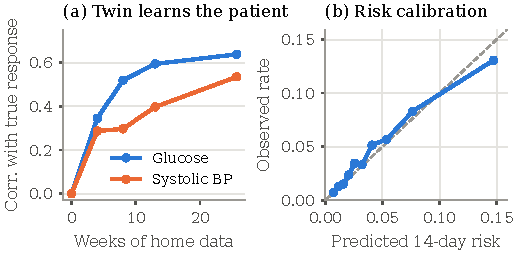
\includegraphics[width=\columnwidth]{figures/fig_twin_calibration.pdf}
\caption{(a) Correlation between the twin's learned drug response and each patient's hidden true response, by weeks of home data (glucose: 292 patients; BP: 478). (b) Reliability curve of the fused risk model.}
\label{fig:twin}
\end{figure}

\textbf{The twin learns the individual.} The EHR prior treats every patient as an average responder, so its correlation with the true response is zero by construction. Fig.~\ref{fig:twin}(a) shows that after 26 weeks the twin's estimate correlates 0.64 (glucose) and 0.54 (BP) with the truth. Pill-box lapses act as natural on/off experiments. The twin's daily forecasts are also calibrated: 95\% of glucose and 97\% of home BP readings fall within its own 2-SD band.

\begin{figure}[t]
\centering
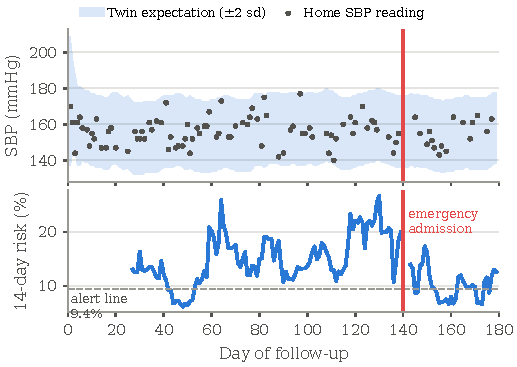
\includegraphics[width=\columnwidth]{figures/fig_case_study.pdf}
\caption{Held-out patient HT00000. Top: home SBP against the twin's expected band. Bottom: weekly-refreshed 14-day risk; red line marks her emergency admission (day 140).}
\label{fig:case}
\end{figure}

\begin{table}[H]
\caption{What-if engine for patient HT00000 (90 days, 16 roll-outs per plan; 56 plans tested)}
\label{tab:whatif}
\centering
\footnotesize
\begin{tabular}{@{}p{3.15cm}cccc@{}}
\toprule
Plan & 14-day & HbA1c & Home & Hypo\\
 & risk & (\%) & SBP & days\\
\midrule
Continue current care & 10.8\% & 8.9 & 157 & 0.1\\
\textbf{Add amlodipine + 2{,}000 steps + adherence support} & \textbf{5.9\%} & \textbf{8.3} & \textbf{148} & \textbf{1.1}\\
Add amlodipine + adherence support & 6.4\% & 8.3 & 148 & 0.5\\
\bottomrule
\end{tabular}
\end{table}

\textbf{Case study:} Patient HT00000 (never used to train the console's model) is a 46-year-old woman from South India with diabetes, hypertension and a prior cardiac event, on metformin, a sulfonylurea and a RAAS blocker, who observes religious fasts. In the 90 days before her emergency her pill-box logged 24 missed doses out of 78, and 17 home readings were $\ge160$\,mmHg. Fig.~\ref{fig:case} shows her risk above the alert line for most of the period, at 19.9\% the day before admission. The record alone would also flag her; what the twin adds is \emph{what to do}. Table~\ref{tab:whatif} shows the top-ranked plan, which nearly halves her simulated risk, together with the cautions it raises for the doctor: ankle oedema with amlodipine and clearing the walking plan after her cardiac event. It also raises her simulated hypoglycaemia days from 0.1 to 1.1, a real concern on a sulfonylurea, so the doctor may prefer the runner-up plan, which has a similar risk (6.4\%) with 0.5 such days.

% =====================================================================
\section{Discussion}
The results support the central claim on synthetic data: fusing daily home data with the clinic record ranks patients better than the record alone, and much better than the threshold rules used today. The gain over the record is small on average (+0.017 AUROC), which matches prior findings that the record carries most of the baseline risk \cite{rajkomar2018}, but it is consistent across seeds and concentrated on the event most sensitive to daily behaviour: severe hypoglycaemia, the commonest preventable harm of sulfonylurea-heavy prescribing during fasting periods \cite{hassanein2022}.

\textbf{Business relevance:} For a programme following 1{,}000 patients, the alert budget translates into about 100 coordinator calls a week, each with a 13\% chance of preceding an event in the next fortnight (vs.\ 4.5\% at random) and a typical week's warning, enough time for a teleconsultation. The what-if engine moves the conversation from ``she is high risk'' to a tested, guarded plan for the doctor, which is the step most remote-monitoring dashboards lack. Because inputs and outputs use HL7 FHIR R4, the system can plug into India's Ayushman Bharat Digital Mission (ABDM) stack rather than adding another silo \cite{mandel2016}.

\textbf{Users and pilot success metrics:} Four groups gain from the output: the care coordinator gets a ranked worklist with plain-language reasons and fasting-season warnings; the physician gets personal drug-response estimates and guarded plan options; the patient gets fewer emergencies and plans that respect fasts and festivals; and the hospital, insurer or employer programme gets fewer avoidable admissions and evidence of care quality. A pilot would judge success on avoidable admissions per 100 patient-years (primary), severe hypoglycaemia episodes in fasting periods, the share of patients reaching HbA1c $<7\%$ and home SBP $<130$\,mmHg at six months, coordinator minutes per patient per month, and alert acceptance rate, which signals both trust and alert fatigue. The adoption path is to embed the model as a SMART-on-FHIR worklist plug-in in the existing coordinator workflow, so patients need no new app, and later to reuse the twin pattern for related conditions such as chronic kidney disease or heart failure by swapping the state equations and event heads.

\textbf{Originality and technical choices:} The separation of a generative twin from a discriminative risk engine was an empirical decision: feeding the twin's coefficients and surprise scores into the risk model \emph{lowered} AUROC by 0.017 ($p\le0.001$), because the raw stream windows already carried the information and 16 extra correlated features led the trees to overfit rare events. The twin's job is therefore to personalise and simulate, not to classify. Choosing the threshold by alert budget, reporting AUPRC and calibration, and testing with a patient-level bootstrap all follow from the rarity of events and from how a care team will actually use the scores. This twin-state effect was not consistent across seeds: the variant averaged $0.721\pm0.013$ against $0.727\pm0.001$ for the fused model and beat it once (seed 11: 0.734 vs.\ 0.728), so we treat the separation as a conservative design choice rather than a proven gain.

\textbf{Limitations:} (i) All data are synthetic; the signal sits where the generator puts it, and real performance is unknown until retrospective validation on paired hospital and device data. (ii) Within-patient timing is only modestly better than chance (0.557 vs.\ 0.500 for the EHR): the model is better at \emph{who} than \emph{when}. (iii) The twin does not recover individual step sensitivity, so activity what-ifs lean on the literature prior. (iv) New-drug effects in the simulator are published averages scaled by the patient's learned response, not causal estimates. (v) Hyper-parameters were chosen between two settings on the same cross-validation; the temporal hold-out and seed sweep are the less optimistic checks. (vi) Fairness across sex, region, income and device type cannot be judged on synthetic data and must be monitored in deployment.

\textbf{Path to real-world validation:} We propose three phases. (1)~A 3--4 month retrospective study on a partner hospital or diabetes-chain programme with paired EHR and device data, accessed through ABDM consent or an ethics-approved protocol, asking in order whether the twin is calibrated on real data, whether its drug-response estimate predicts the HbA1c change after a later dose change, and whether fused beats EHR-only on admissions with patient-level bootstrap intervals; the analysis plan and alert budget are fixed before unblinding to avoid the model-selection optimism noted above. (2)~A six-month silent prospective run, where the twin scores live patients unseen by clinicians, to measure calibration drift, lead time and alerts per clinician per day. (3)~A cluster-randomised clinician-in-the-loop pilot with avoidable admissions as the primary outcome, logging every recommendation against the clinician's decision. Software that informs treatment is likely a medical device under India's Medical Devices Rules 2017 (Central Drugs Standard Control Organisation, CDSCO), so phases 2 and 3 would form its clinical evidence.

\textbf{Ethics, privacy and equity:} The prototype uses no real personal data. In deployment, data would enter only through ABDM consent artefacts that name the purpose (care management) and duration, in line with India's Digital Personal Data Protection Act 2023. The system uses daily summaries only (no GPS, raw sensor streams or diet photos), keeps per-patient twin state that can be erased with the source data, and needs a separate consent purpose to retrain. Every plan is labelled for clinician review and nothing is sent to a patient automatically. Because device access varies across income, gender and rural or urban settings, a programme should support glucometer-only and SMS or interactive voice response (IVR) patients, treat missing data as a signal, report performance by subgroup, and never deprioritise a patient for sending fewer readings. This matters because proxy targets can encode inequity: a widely used US care-management algorithm under-served Black patients by using past cost as a proxy for need \cite{obermeyer2019}.

% =====================================================================
\section{Reproducibility}
\label{sec:repro}
The repository \url{\RepoURL} holds the code, the cleaned modelling dataset (in \texttt{data/processed/}), a sample of every raw table, the generated results and this report's source. To replicate the core results:
\begin{enumerate}
\item \texttt{git clone} the repository and run \texttt{pip install -r requirements.txt} (Python $\ge$3.10; tested versions are pinned in \texttt{requirements-lock.txt}).
\item Run \texttt{python run\_pipeline.py}. It regenerates the cohort (seed 2026), runs the twin, trains and evaluates every model, runs the seed sweep, builds the clinician console and writes \texttt{docs/RESULTS.md} (about 4 minutes on a laptop CPU; \texttt{-{}-quick} runs in about 1 minute).
\item Run \texttt{pytest} (16 tests: determinism, no future leakage, label windows, twin recovery, guardrails, FHIR round-trip) and \texttt{python report/make\_figures.py} for the figures in this paper, and \texttt{python report/extra\_analyses.py} for Table~\ref{tab:op} and the SHAP ranking.
\end{enumerate}
The pipeline is deterministic: a fresh run reproduced every number in this report exactly. GitHub Actions runs the tests and a reduced pipeline on every push.

\subsection{AI Use Declaration}
\label{sec:ai}
% TEAM: list here any other AI tools you used while writing the pipeline code
% (e.g. ChatGPT, Copilot), and keep AI-generated content below 20% after your own edits.
Claude (Anthropic) was used to draft and copy-edit this report from the team's code and pipeline outputs, to write the figure script (\texttt{report/make\_figures.py}) and to reorganise the repository documentation. Every number was regenerated by the pipeline and checked by the team, and the text was reviewed and rewritten by the authors. AI-generated content in the final submission is kept below 20\% as required.

% =====================================================================
\section{Conclusion}
HridayTwin shows that a simple, identifiable patient twin combined with a gradient-boosted risk engine can turn between-visit home data into a ranked, explained call list and a short list of tested care plans. On a 1{,}200-patient synthetic cohort, home data improved risk ranking over the clinic record (AUROC 0.726 vs.\ 0.708) and most clearly for severe hypoglycaemia (0.943 vs.\ 0.907), with a week's median warning at a workable alert load. Future work is to validate on retrospective paired EHR and device data from an Indian hospital under ethics approval, run a silent prospective pilot, score daily with a shorter horizon to improve timing, and test the plan recommendations against what clinicians actually choose.

\section*{Acknowledgment}
The authors thank the faculty of the Advanced Machine Learning for Business Transformation course at Goa Institute of Management for their guidance and feedback.

% =====================================================================
\begin{thebibliography}{00}
\bibitem{anjana2023} R. M. Anjana \textit{et al.}, ``Metabolic non-communicable disease health report of India: the ICMR-INDIAB national cross-sectional study (ICMR-INDIAB-17),'' \textit{Lancet Diabetes Endocrinol.}, vol. 11, no. 7, pp. 474--489, Jul. 2023.
\bibitem{bjornsson2020} B. Bj\"{o}rnsson \textit{et al.}, ``Digital twins to personalize medicine,'' \textit{Genome Med.}, vol. 12, Art. no. 4, 2020.
\bibitem{corral2020} J. Corral-Acero \textit{et al.}, ``The `Digital Twin' to enable the vision of precision cardiology,'' \textit{Eur. Heart J.}, vol. 41, no. 48, pp. 4556--4564, Dec. 2020.
\bibitem{katsoulakis2024} E. Katsoulakis \textit{et al.}, ``Digital twins for health: a scoping review,'' \textit{npj Digit. Med.}, vol. 7, Art. no. 77, Mar. 2024.
\bibitem{man2014} C. D. Man \textit{et al.}, ``The UVA/PADOVA type 1 diabetes simulator: new features,'' \textit{J. Diabetes Sci. Technol.}, vol. 8, no. 1, pp. 26--34, 2014.
\bibitem{rajkomar2018} A. Rajkomar \textit{et al.}, ``Scalable and accurate deep learning with electronic health records,'' \textit{npj Digit. Med.}, vol. 1, Art. no. 18, 2018.
\bibitem{ruan2020} Y. Ruan \textit{et al.}, ``Predicting the risk of inpatient hypoglycemia with machine learning using electronic health records,'' \textit{Diabetes Care}, vol. 43, no. 7, pp. 1504--1511, Jul. 2020.
\bibitem{kalman1960} R. E. Kalman, ``A new approach to linear filtering and prediction problems,'' \textit{J. Basic Eng.}, vol. 82, no. 1, pp. 35--45, 1960.
\bibitem{durbin2012} J. Durbin and S. J. Koopman, \textit{Time Series Analysis by State Space Methods}, 2nd ed. Oxford, U.K.: Oxford Univ. Press, 2012.
\bibitem{friedman2001} J. H. Friedman, ``Greedy function approximation: a gradient boosting machine,'' \textit{Ann. Statist.}, vol. 29, no. 5, pp. 1189--1232, 2001.
\bibitem{ke2017} G. Ke \textit{et al.}, ``LightGBM: a highly efficient gradient boosting decision tree,'' in \textit{Proc. Adv. Neural Inf. Process. Syst. (NeurIPS)}, 2017, pp. 3146--3154.
\bibitem{pedregosa2011} F. Pedregosa \textit{et al.}, ``Scikit-learn: machine learning in Python,'' \textit{J. Mach. Learn. Res.}, vol. 12, pp. 2825--2830, 2011.
\bibitem{lundberg2017} S. M. Lundberg and S.-I. Lee, ``A unified approach to interpreting model predictions,'' in \textit{Proc. Adv. Neural Inf. Process. Syst. (NeurIPS)}, 2017, pp. 4765--4774.
\bibitem{walonoski2018} J. Walonoski \textit{et al.}, ``Synthea: an approach, method, and software mechanism for generating synthetic patients and the synthetic electronic health care record,'' \textit{J. Am. Med. Inform. Assoc.}, vol. 25, no. 3, pp. 230--238, 2018.
\bibitem{nathan2008} D. M. Nathan \textit{et al.}, ``Translating the A1C assay into estimated average glucose values,'' \textit{Diabetes Care}, vol. 31, no. 8, pp. 1473--1478, 2008.
\bibitem{kwong2018} J. C. Kwong \textit{et al.}, ``Acute myocardial infarction after laboratory-confirmed influenza infection,'' \textit{N. Engl. J. Med.}, vol. 378, no. 4, pp. 345--353, 2018.
\bibitem{hassanein2022} M. Hassanein \textit{et al.}, ``Diabetes and Ramadan: practical guidelines 2021,'' \textit{Diabetes Res. Clin. Pract.}, vol. 185, Art. no. 109185, 2022.
\bibitem{saito2015} T. Saito and M. Rehmsmeier, ``The precision-recall plot is more informative than the ROC plot when evaluating binary classifiers on imbalanced datasets,'' \textit{PLoS ONE}, vol. 10, no. 3, Art. no. e0118432, 2015.
\bibitem{vancalster2019} B. Van Calster \textit{et al.}, ``Calibration: the Achilles heel of predictive analytics,'' \textit{BMC Med.}, vol. 17, Art. no. 230, 2019.
\bibitem{mandel2016} J. C. Mandel \textit{et al.}, ``SMART on FHIR: a standards-based, interoperable apps platform for electronic health records,'' \textit{J. Am. Med. Inform. Assoc.}, vol. 23, no. 5, pp. 899--908, 2016.
\bibitem{obermeyer2019} Z. Obermeyer \textit{et al.}, ``Dissecting racial bias in an algorithm used to manage the health of populations,'' \textit{Science}, vol. 366, no. 6464, pp. 447--453, Oct. 2019.
\end{thebibliography}

\end{document}
